\let\cleardoublepage\clearpage
\chapter{Empirical Evaluation}
\label{chapter:Evaluation}

Main goal of this chapter is to assess how much is our IE checker
is efficient in terms of the count that it is able to detect true-positives,
false-negatives, false-positives, execution times and also its ability to fix
the detected bugs. Along with this, highlighting the research work that has
been carried out in this thesis. For the purpose of evaluation, we have used
the IE checker and the Juliet test cases CWE-524/535/536. All the results
from this evaluation will be represented in tables and also in graphs.



\section{Test Setup}

In order to fix the detected IE bugs, developed refactoring tool was used
for generating the two types of patches and then inserting in the
code program. Exisiting IE checker[ref] was used in order to detect the 
IE bugs in the code programs and also to classify the bug depending on the
bug description and its unique ID. Used 64-bit Linux Kernel 3.13.0-32.57, Intel i5-
3230 CPU @ 2.60GHz × 4 was used as a test system. Calculated the times needed to generated
all the patches and also the total time for detecting the bug. Measured
the times in milliseconds.


\section{Methodology}

CWE- 526/534/535 were used as the test cases for running our already existing IE checker
because these test cases contain the bugs for which the IE checker was built.
All the test cases were also publicly online available in the 
Juliet test suite [ref]. The number of test programs present in CWE-526 are 18 Test Programs(TPr),
CWE-534 has 36 TPr and CWE-536 has 36 TPr. All these test programs CWE-526/534/535 were 
exported in to the eclipse workspace by already created Eclipse CDT project instance.

After all the test programs were imported into the Eclipse CDT workspace,
the existing IE checker which is an eclipse JDT plugin was made to 
run automatically for each test program available in the workspace.
This can be done by selecting the submenu "Run C/C++ Code analysis" after
right clicking on the selected test program. The following time were measured
and represented in the respective tables: time for running the checker for detecting the bug was
measured [ref], time for refactoring[], execution time for the test programs which belong
to the test case, these were measured for  all the analyzed test programs.
Also the number of true positives, false positives, true negatives and false negatives
were are also calculated and reperesented in the table[]. 

[// here write how all the values in the table were calculated]



It was already know the number of test programs that should have the bug marker icon in the
test program after running the IE checker using static analysis and 
also the count on how many should not have the bug marker icon ( 5 out of 90 test
programs will not contain the bug icon since it was not possible for running the
static analysis). Usually a bug icon is similar to the image of a bug and the description of the
bug is shown in the console view with a triangle symbol with an exclamation mark inside it.

Different types of messages that can be seen are:
\begin{figure}[!htb]
\centering
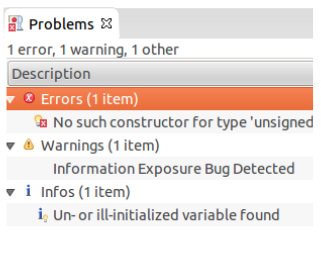
\includegraphics[width=0.5\textwidth]{png/Types.png}
\caption{Types of possible messages}
\label{fig:types}
\end{figure}\\

\begin{enumerate}
\item Errors
\item Warnings
\item Infos
\end{enumerate}

Errors are represented with red circle with a cross inside icon, Warnings are represented
with a traingle and exclamation mark inside icon, infos is represented with i symbol icon.
In this IE checker we do not use errors and infos but only the warnings
where the bug descripted will be displayed in the console view of
the Eclipse CDT instance after running the IE checker and detecting
the bugs as shown in figure~\ref{fig:types}. Therefore once the bugs are
detected and the bug mark icon is placed, one can see the traingle icon 
with exclamation mark inside in the console view. Once we click on the
message that has been generated by the Information exposure bug report
represented in figure~\ref{fig:types} then the cursor will be pointing
to the line number where the bug was found. There are different modes in which
the IE checker can be configured in order to launch the checker as shown 
in figure~\ref{fig:modes}. This bug triggering modes can be very useful during the 
software development by giving a chance to the developer on how to control
and when should eclipse trigger the bug detection analysis. This will help the
developer to avoid insertion of bugs during the software development.
\begin{figure}[!htb]
\centering
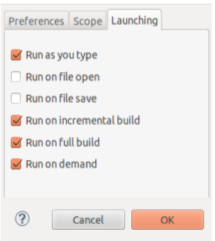
\includegraphics[width=0.4\textwidth]{png/modes.png}
\caption{Different modes}
\label{fig:modes}
\end{figure}\\

\section{Results and Constraints}



\begin{table}[h!]
\centering
 \begin{tabular}{||c |c |c |c |c| c|c||} 
 \hline
 \textbf{Test Program} & \textbf{PGT} & \textbf{TT} & \textbf{No; of Paths} & \textbf{IP}& \textbf{Total no; of nodes}&
 \textbf{BDT}\\ [0.5ex] 
 \hline\hline
 CWE526-env-01 & 0.014 & 7.442 & 8 & 0& 250&7.428\\ 
 \hline
CWE526-env-02 & 0.02 & 4.082 & 12&0& 498&4.062\\ 
 \hline
 CWE526-env-03 & 0.013 & 3.603 & 12&0& 498&3.59\\ 
 \hline
 CWE526-env-04 & 0.017 & 3.306 & 12&0& 498&3.289\\ 
 \hline
 CWE526-env-05 & 0.017 & 3.456 & 12&0& 498&3.439\\ 
 \hline
 CWE526-env-06 & 0.01 & 3.455 & 12&0& 498&3.445\\ 
 \hline
 CWE526-env-07 & 0.011 & 3.386 & 12&0& 500&3.375\\ 
 \hline
 CWE526-env-08 & 0.01 & 3.169 & 12&0& 564&3.159\\ 
 \hline
 CWE526-env-09 & 0.008 & 3.241 & 12&0& 498&3.233\\ 
 \hline
 CWE526-env-10 & 0.012 & 3.373 & 12&0&498&3.361 \\ 
 \hline
 CWE526-env-11 & 0.014 & 3.207 & 12&0&564&3.193 \\ 
 \hline
 CWE526-env-12 & 0.017 & 3.116 &20&0& 1001&3.099\\ 
 \hline
 CWE526-env-13 & 0.013 & 3.236 & 12&0& 498&3.223\\ 
 \hline
 CWE526-env-14 & 0.014 & 3.239 & 12&0& 498&3.225\\ 
 \hline
 CWE526-env-15 & 0.014 & 3.272 & 12&0&507&3.258\\ 
 \hline
  CWE526-env-16 & 0.005 & 3.182 & 10&0& 356&3.177\\ 
 \hline
  CWE526-env-17 & 0.005 & 3.303 & 12&0& 533&3.298\\ 
 \hline
  CWE526-env-18 & 0.0 & 0 & 0&0& 0&0\\ 
 \hline
 \hline
\end{tabular}
\caption{Measured values of CWE-526}
\label{table:times}
\end{table}


\begin{table}[h!]
\centering
 \begin{tabular}{||c |c |c |c |c| c||} 
 \hline
 \textbf{Testcase} & \textbf{RT} & \textbf{TT} & \textbf{No; of Paths} & \textbf{IP}& \textbf{Total no; of nodes} \\ [0.5ex] 
 \hline\hline
 CWE534-debug-char-01 & 0.004 & 5.644 & 87 & 0& 7560\\ 
 \hline
CWE534-debug-char-02 & 0.043 &  9.688 & 372&0& 48645\\ 
 \hline
 CWE534-debug-char-03 & 0.01& 8.649 & 372&0& 48645\\ 
 \hline
 CWE534-debug-char-04 & 0.013 & 8.62 & 370&0& 48552\\ 
 \hline
 CWE534-debug-char-05 & 0.016 & 8.487 & 372&0& 48645\\ 
 \hline
 CWE534-debug-char-06 & 0.015 & 8.264& 371&0& 48609\\ 
 \hline
 CWE534-debug-char-07 & 0.014 & 8.352 & 372&0& 48645\\ 
 \hline
 CWE534-debug-char-08 & 0.018 &6.421 & 198&0& 30141\\ 
 \hline
 CWE534-debug-char-09 & 0.051 &10.177 &372&0& 48645\\ 
 \hline
 CWE534-debug-char-10 & 0.022 & 7.894& 278&0&36495 \\ 
 \hline
 CWE534-debug-char-11 & 0.017 &8.891& 372&0&51699 \\ 
 \hline
 CWE534-debug-char-12 & 0.007 & 7.363 &308&0& 32341\\ 
 \hline
 CWE534-debug-char-13 & 0.015 &48.654 & 372&0& 48645\\ 
 \hline
 CWE534-debug-char-14 & 0.02 & 8.517 & 372&0& 48645\\ 
 \hline
 CWE534-debug-char-15 & 0.011 & 8.555 & 372&0&49014\\ 
 \hline
  CWE534-debug-char-16 & 0.003 &4.266 & 92&0& 8551\\ 
 \hline
  CWE534-debug-char-17 & 0.002 & 3.989 & 57&0& 5905\\ 
 \hline
  CWE534-debug-char-18 & 0.0 & 0 & 0&0& 0\\ 
  \hline
  CWE534-debug-wchar-01 & 0.003 &3.846 &61 & 0& 5816\\ 
 \hline
CWE534-debug-wchar-02 & 0.005 & 5.726 & 204&0& 29470\\ 
 \hline
 CWE534-debug-wchar-03 & 0.005 &5.662 & 204&0& 29470\\ 
 \hline
 CWE534-debug-wchar-04 & 0.019 & 5.73 & 204&0& 29470\\ 
 \hline
 CWE534-debug-wchar-05 & 0.004 & 5.806 & 204&0& 29470\\ 
 \hline
 CWE534-debug-wchar-06 & 0.005 & 5.711 & 204&0& 29470\\ 
 \hline
 CWE534-debug-wchar-07 & 0.006 & 5.666 & 204&0& 29470\\ 
 \hline
 CWE534-debug-wchar-08 & 0.008 & 5.619 & 204&0& 31084\\ 
 \hline
 CWE534-debug-wchar-09 & 0.007 & 5.674 & 204&0& 29470\\ 
 \hline
 CWE534-debug-wchar-10 & 0.003 & 5.732 & 202&0&29276 \\ 
 \hline
 CWE534-debug-wchar-11 & 0.005 & 5.718 &204&0&31084 \\ 
 \hline
 CWE534-debug-wchar-12 & 0.003 &6.337 &211&0& 24400\\ 
 \hline
 CWE534-debug-wchar-13 & 0.004 & 5.903 & 203&0& 29404\\ 
 \hline
 CWE534-debug-wchar-14 & 0.005 & 5.548 & 204&0& 29470\\ 
 \hline
 CWE534-debug-wchar-15 & 0.003 & 5.779 & 199&0&29323\\ 
 \hline
  CWE534-debug-wchar-16 & 0.001 & 3.847 & 66&0& 6608\\ 
 \hline
  CWE534-debug-wchar-17 & 0.002 & 4.027 & 78&0& 8752\\ 
 \hline
  CWE534-debug-wchar-18 & 0.0 & 0 & 0&0& 0\\
 \hline
 \hline
\end{tabular}
\caption{Measured values of CWE-534}
\label{table:times}
\end{table}


\begin{table}[h!]
\centering
 \begin{tabular}{||c |c |c |c |c| c||} 
 \hline
 \textbf{Testcase} & \textbf{RT} & \textbf{TT} & \textbf{No; of Paths} & \textbf{IP}& \textbf{Total no; of nodes} \\ [0.5ex] 
 \hline\hline
 CWE535-shell-char-01 & 0.001 & 3.946 &67 & 0&5239\\ 
 \hline
CWE535-shell-char-02 & 0.014 & 7.316 & 288&0& 33700 \\
 \hline
 CWE535-shell-char-03 & 0.013 & 7.379 & 288&0& 33700\\ 
 \hline
 CWE535-shell-char-04 & 0.015 & 7.472 & 288&0& 33700\\ 
 \hline
 CWE535-shell-char-05 & 0.025 & 7.336 & 288&0& 33700\\ 
 \hline
 CWE535-shell-char-06 & 0.014 & 7.41 & 288&0& 33700\\ 
 \hline
 CWE535-shell-char-07 & 0.017 & 7.257 & 288&0& 33700\\ 
 \hline
 CWE535-shell-char-08 & 0.014 & 7.392 & 288&0& 36070\\ 
 \hline
 CWE535-shell-char-09 & 0.018 & 7.367 & 288&0& 33700\\ 
 \hline
 CWE535-shell-char-10 & 0.005 & 4.797 & 112&0&12794 \\ 
 \hline
 CWE535-shell-char-11 & 0.019 & 7.25 & 288&0&36070 \\ 
 \hline
 CWE535-shell-char-12 &0.007  & 6.509 &236&0& 22707\\ 
 \hline
 CWE535-shell-char-13 &0.012  & 7.285 & 288&0& 33700\\ 
 \hline
 CWE535-shell-char-14 & 0.018 & 7.547 & 288&0& 33700\\ 
 \hline
 CWE535-shell-char-15 & 0.015 & 6.921 &254&0&29867\\ 
 \hline
  CWE535-shell-char-16 & 0.004 & 4.223 & 71&0& 6007\\ 
 \hline
  CWE535-shell-char-17 & 0.003 &4.491 & 92&0& 8910\\ 
 \hline
  CWE535-shell-char-18 & 0.0 & 0.0 & 0&0& 0\\ 
  \hline
  CWE535-shell-wchar-01 & 0.001 & 3.645 &48 & 0& 4198\\ 
 \hline
CWE535-shell-wchar-02 & 0.005 & 5.223 & 165&0& 21568\\ 
 \hline
 CWE535-shell-wchar-03 & 0.006 & 5.208 & 165&0& 21568\\ 
 \hline
 CWE535-shell-wchar-04 & 0.005 & 5.28 & 165&0& 21568\\ 
 \hline
 CWE535-shell-wchar-05 & 0.005 &5.248 & 165&0& 21568\\ 
 \hline
 CWE535-shell-wchar-06 & 0.008 & 5.47 & 165&0& 21568\\ 
 \hline
 CWE535-shell-wchar-07 & 0.006& 5.216 & 165&0& 21568\\ 
 \hline
 CWE535-shell-wchar-08 & 0.007 & 5.543 & 165&0& 22876\\ 
 \hline
 CWE535-shell-wchar-09 & 0.005 & 5.24 & 165&0& 21568\\ 
 \hline
 CWE535-shell-wchar-10 & 0.008 & 5.036 & 165&0&21568 \\ 
 \hline
 CWE535-shell-wchar-11 & 0.007 & 5.326 & 165&0&22876 \\ 
 \hline
 CWE535-shell-wchar-12 & 0.004 & 5.245 &170&0& 18037\\ 
 \hline
 CWE535-shell-wchar-13 & 0.01 &5.218 & 165&0& 21568\\ 
 \hline
 CWE535-shell-wchar-14 & 0.006 & 5.521 &170&0& 21568\\ 
 \hline
 CWE535-shell-wchar-15 & 0.005 & 5.401 & 165&0&21730\\ 
 \hline
  CWE535-shell-wchar-16 & 0.001 & 3.914 & 165&0& 4922\\ 
 \hline
  CWE535-shell-wchar-17 & 0.006 & 5.561 & 165&0& 21568\\ 
 \hline
  CWE535-shell-wchar-18 & 0.0 & 0 & 0&0& 0\\
 \hline
 \hline
\end{tabular}
\caption{Measured values of CWE-535}
\label{table:times}
\end{table}
\section{Correctness validation}


\section{Correctness validation}
all the validations 
 
\section{Efficiency and Overhead}
about the tool Efficiency.

\section{Program Behaviour}
Program behaviour tells us if the newly inserted code patch changes the
behaviour of the program or not. Here program behaviour means
that the inserted code patches should not be able to influence the
already existing program paths. The abbrevation form the table
IPa(Influencible paths), IP(Influencible Programs), \% Ratio represents
the ratio between the total number of programs to the total number of
influencible programs which contains atleast one influencible path.
Based on the decision made at the time for running the localizer,
which means there exits a not-in-place fix also. So after finding the 
not-in-place fix and inserting the code patch into the program form
refactoring then the program paths are then verified in order 
to check if the inserted code patch would change the program behaviour
or not. After verifying for the influencible paths, if it finds any such
influencible paths then the refactorings are not at all generated and
the decision is left to the programmer to refactor the code 
or not. This way the change of program behaviour can be avoided by not
proposing the refactorings at all.


\section{Usefulness of the generated Patches}
Usefulness of the generated patches.

\chapter{Discussion}
\label{chapter:Discussion}

\section{Limitations}
limitations of the tool and approach.

\section{Applications}
Where can this be applied.

\section{Future Work}
about the Future work.

\chapter{Summary and Conclusion}
\label{chapter:Conclusion}